\documentclass[journal,twoside]{IEEEtran}
\usepackage{amsmath,amssymb,amsfonts}
\usepackage{graphicx}
\usepackage{booktabs}
\usepackage{multirow}
\usepackage{xcolor}
\usepackage{cite}
\usepackage[hidelinks]{hyperref}

\newcommand{\pbs}{\textsc{pbs}}
\newcommand{\ppo}{\textsc{PPO}}
\newcommand{\trpo}{\textsc{TRPO}}
\newcommand{\grpo}{\textsc{GRPO-C}}

\begin{document}

\title{Reward Paradigm Design for Robot Policy Optimization: Sparse, Dense,
Potential-Based and Curriculum Rewards across Optimizer Families}

\author{Aitachi%
\thanks{Companion paper to the algorithm-comparison study; all reward
functions, audits and raw logs are in the open suite
https://github.com/aitachi/Reinforcement-Learning-Policy.}}

\maketitle

\begin{abstract}
Reward design remains the least standardized component of robot
reinforcement learning: the same task admits many ad-hoc reward functions,
and algorithm papers rarely report which reward signal their conclusions
rest on. We formalize four reward \emph{paradigms}---sparse outcome,
engineered dense, potential-based shaping (PBS), and curriculum
annealing---and instantiate each on three robot tasks (obstacle navigation,
legged locomotion, reach--grasp--lift), yielding twelve fully specified
reward functions with per-term audits. We train three representative
optimizers (\ppo{}-Clip, \trpo{}, \grpo{}) under every paradigm
(3 tasks $\times$ 4 paradigms $\times$ 3 seeds $\times$ 3 algorithms) and
explain the observed outcome structure mechanistically: where potential-based
shaping preserves optimal policies as theory predicts, where it silently
distorts them under discounting (locomotion PBS: 0.12--0.13 vs dense
0.62--0.68), where dense engineering invites reward-hacking (we document
and fix a grasp-boundary flicker exploit that farmed event bonuses at
0.59/step), and why group-outcome baselines invert the usual sparse-reward
advice (GRPO under sparse 0.11 beats its dense 0.02 on locomotion). We
distill the results into design guidelines and release the paradigm
library.
\end{abstract}

\begin{IEEEkeywords}
reward design, reward shaping, potential-based rewards, curriculum
learning, reward hacking, reinforcement learning, robot learning
\end{IEEEkeywords}

\section{Introduction}
A reinforcement-learning agent does not optimize the task; it optimizes the
reward. In robot control the gap between the two is engineered away by
hand: progress bonuses, energy penalties, milestone rewards, curricula.
The literature offers partial theory---potential-based shaping preserves
optimal policies exactly~\cite{ng1999policy}, and curriculum scheduling
changes the effective task difficulty~\cite{bengio2009curriculum}---but
practical guidance is fragmented across papers, each typically evaluating
one reward with one algorithm.

Meanwhile, the LLM post-training community trains on \emph{verifiable
outcome} rewards, where group-relative baselines (GRPO~\cite{shao2024grpo},
DAPO~\cite{yu2025dapo}) handle the extreme sparsity by comparing whole
episodes. Whether the resulting optimizers change which reward paradigm is
learnable on robots is untested.

This paper makes three contributions:
\begin{enumerate}
\item A complete, audited reward paradigm library for three robot tasks:
twelve reward functions specified to the coefficient
(\S\ref{sec:library}), with per-term telemetry that exposes dominance and
hacking;
\item A controlled paradigm $\times$ algorithm study
(3 algorithms $\times$ 4 paradigms $\times$ 3 tasks $\times$ 3 seeds,
\S\ref{sec:results});
\item Mechanistic explanations backed by term audits and a documented
reward-hacking case study (grasp-flicker farming, \S\ref{sec:hacking}),
distilled into design guidelines (\S\ref{sec:guidelines}).
\end{enumerate}

\section{Background and Theory}
\label{sec:theory}
\subsection{Problem setting}
MDP $(\mathcal S,\mathcal A,P,r,\gamma)$; a reward \emph{paradigm} is a
mapping from task signals (distances, events, efforts) exposed by the
environment to a scalar stream. We require paradigms to be algorithm-
agnostic: the same stream feeds value-based critics or group-outcome
baselines.

\subsection{Potential-based shaping}
For $F(s,s')=\gamma\phi(s')-\phi(s)$, the shaped objective's greedy policy
ordering is unchanged for any bounded $\phi$~\cite{ng1999policy}; with
$\gamma<1$ the \emph{optimal} policy under the shaped (discounted) return
is preserved only when $\phi$ is the optimal value function up to constant
scaling---practical hand-designed $\phi$ inherits a distortion we quantify
empirically. PBS converts sparse tasks into dense gradients \emph{without}
changing the apparent task; the catch is that it adds no information, only
re-weights temporal credit.

\subsection{Dense engineering and its failure modes}
Engineered multi-term rewards inject task knowledge but admit degenerate
optima: term farming (an agent maximizes one term against task intent),
plateau traps (zero gradient after partial achievement), and
dominance imbalance (one term drowns the others). We audit each term
online and report mean contributions; abrupt single-term dominance is the
operational signature of farming.

\subsection{Curriculum}
Curricula interpolate task difficulty $d(p)$ and reward $r_p$ with
training progress $p$. Two failure modes: schedule too fast (collapse to
the terminal task's sparse regime) and reward non-stationarity
(non-stationary objective for on-policy methods).

\section{The Paradigm Library}
\label{sec:library}
Tables~\ref{tab:nav-r}--\ref{tab:grasp-r} give the complete specifications
per task; coefficients were selected by a small pre-study (grid of 3 values
for the dominant coefficient) and frozen before the main runs.

\begin{table}[t]
\centering
\caption{E1 navigation reward paradigms.}
\label{tab:nav-r}
\begin{tabular}{lp{5.4cm}}
\toprule
paradigm & specification \\
\midrule
sparse & $3\,\mathbb 1[\text{goal}]-1\,\mathbb 1[\text{collision}]
-0.01\mathbb 1[\text{timeout}]$ \\
dense & $2.5(d_{t-1}-d_t)-0.01-0.02\|a\|^2+3\,\mathbb 1[\text{goal}]
-\mathbb 1[\text{collision}]$ \\
pbs & sparse $+\,\gamma\phi(s_t)-\phi(s_{t-1})$,
$\phi=-4\,d$ (distance to goal) \\
curriculum & $(1-w)\,r_{dense}+w\,r_{sparse}$,
$w=(p/0.8)^{1.5}$; obstacles $1{\to}8$, goal span grows with $p$ \\
\bottomrule
\end{tabular}
\end{table}

\begin{table}[t]
\centering
\caption{E2 locomotion reward paradigms ($v_x$ clipped to $[-2,2]$, target
speed $v^*$).}
\label{tab:hop-r}
\begin{tabular}{lp{5.4cm}}
\toprule
paradigm & specification \\
\midrule
sparse & $0.01\,\mathbb 1[\text{alive}]
+\mathbb 1[\text{end}]\big(\tfrac{x_T-x_0}{3}-2\,\mathbb 1[\text{fall}]\big)
+0.5\,\mathbb 1[\text{survive}]$ \\
dense & $1.5\min(v_x,v^*)-0.6|v_x-v^*|+0.5\,\mathbb 1[\text{alive}]
-2\,\mathbb 1[\text{fall}]-0.004\|a\|^2$ \\
pbs & sparse $+\,\gamma\phi_t-\phi_{t-1}$,
$\phi=2\,v_x^{clip}+0.5\,\mathbb 1[\text{alive}]+0.5\,\mathrm{clip}(y)$ \\
curriculum & dense with $v^*(p)=0.4\to1.2$ over $p\le0.7$ \\
\bottomrule
\end{tabular}
\end{table}

\begin{table}[t]
\centering
\caption{E3 grasp reward paradigms ($h$ object height, $d_{eo}$ EE--object
distance, milestones $h\in\{0.05,0.10,0.14\}$).}
\label{tab:grasp-r}
\begin{tabular}{lp{5.4cm}}
\toprule
paradigm & specification \\
\midrule
sparse & $3\,\mathbb 1[\text{lift}]-0.5\,\mathbb 1[\text{drop}]-0.01$ \\
dense & $3(d_{t-1}-d_t)+8\,\Delta h^+\,\mathbb 1[\text{grasp}]
+2\,\mathbb 1[\text{first grasp}]
+\sum_m \mathbb 1[h\!\uparrow\! m]
+5\,\mathbb 1[\text{lift}]-0.5\,\mathbb 1[\text{drop}]-0.02-0.005\|a\|^2$ \\
pbs & sparse $+\,\gamma\phi_t-\phi_{t-1}$,
$\phi=-4\,d_{eo}+2\,\mathbb 1[\text{grasp}]\min(h,0.18)$ \\
curriculum & $(1-w)r_{dense}+w\,r_{sparse}$, $w=(p/0.8)^{1.5}$;
spawn corridor widens with $p$ \\
\bottomrule
\end{tabular}
\end{table}

\section{Experimental Setup}
Identical to the companion study: 2$\times$128 MLPs, fixed budgets
(E1 400k, E2 600k, E3 500k env steps), 3 seeds, deterministic evaluation on
64 fresh episodes at full difficulty every 20k steps. Paradigm comparability
is preserved by reporting task-native success metrics (never the reward
scale).

\section{Results}
\label{sec:results}

\begin{figure*}[t]
\centering
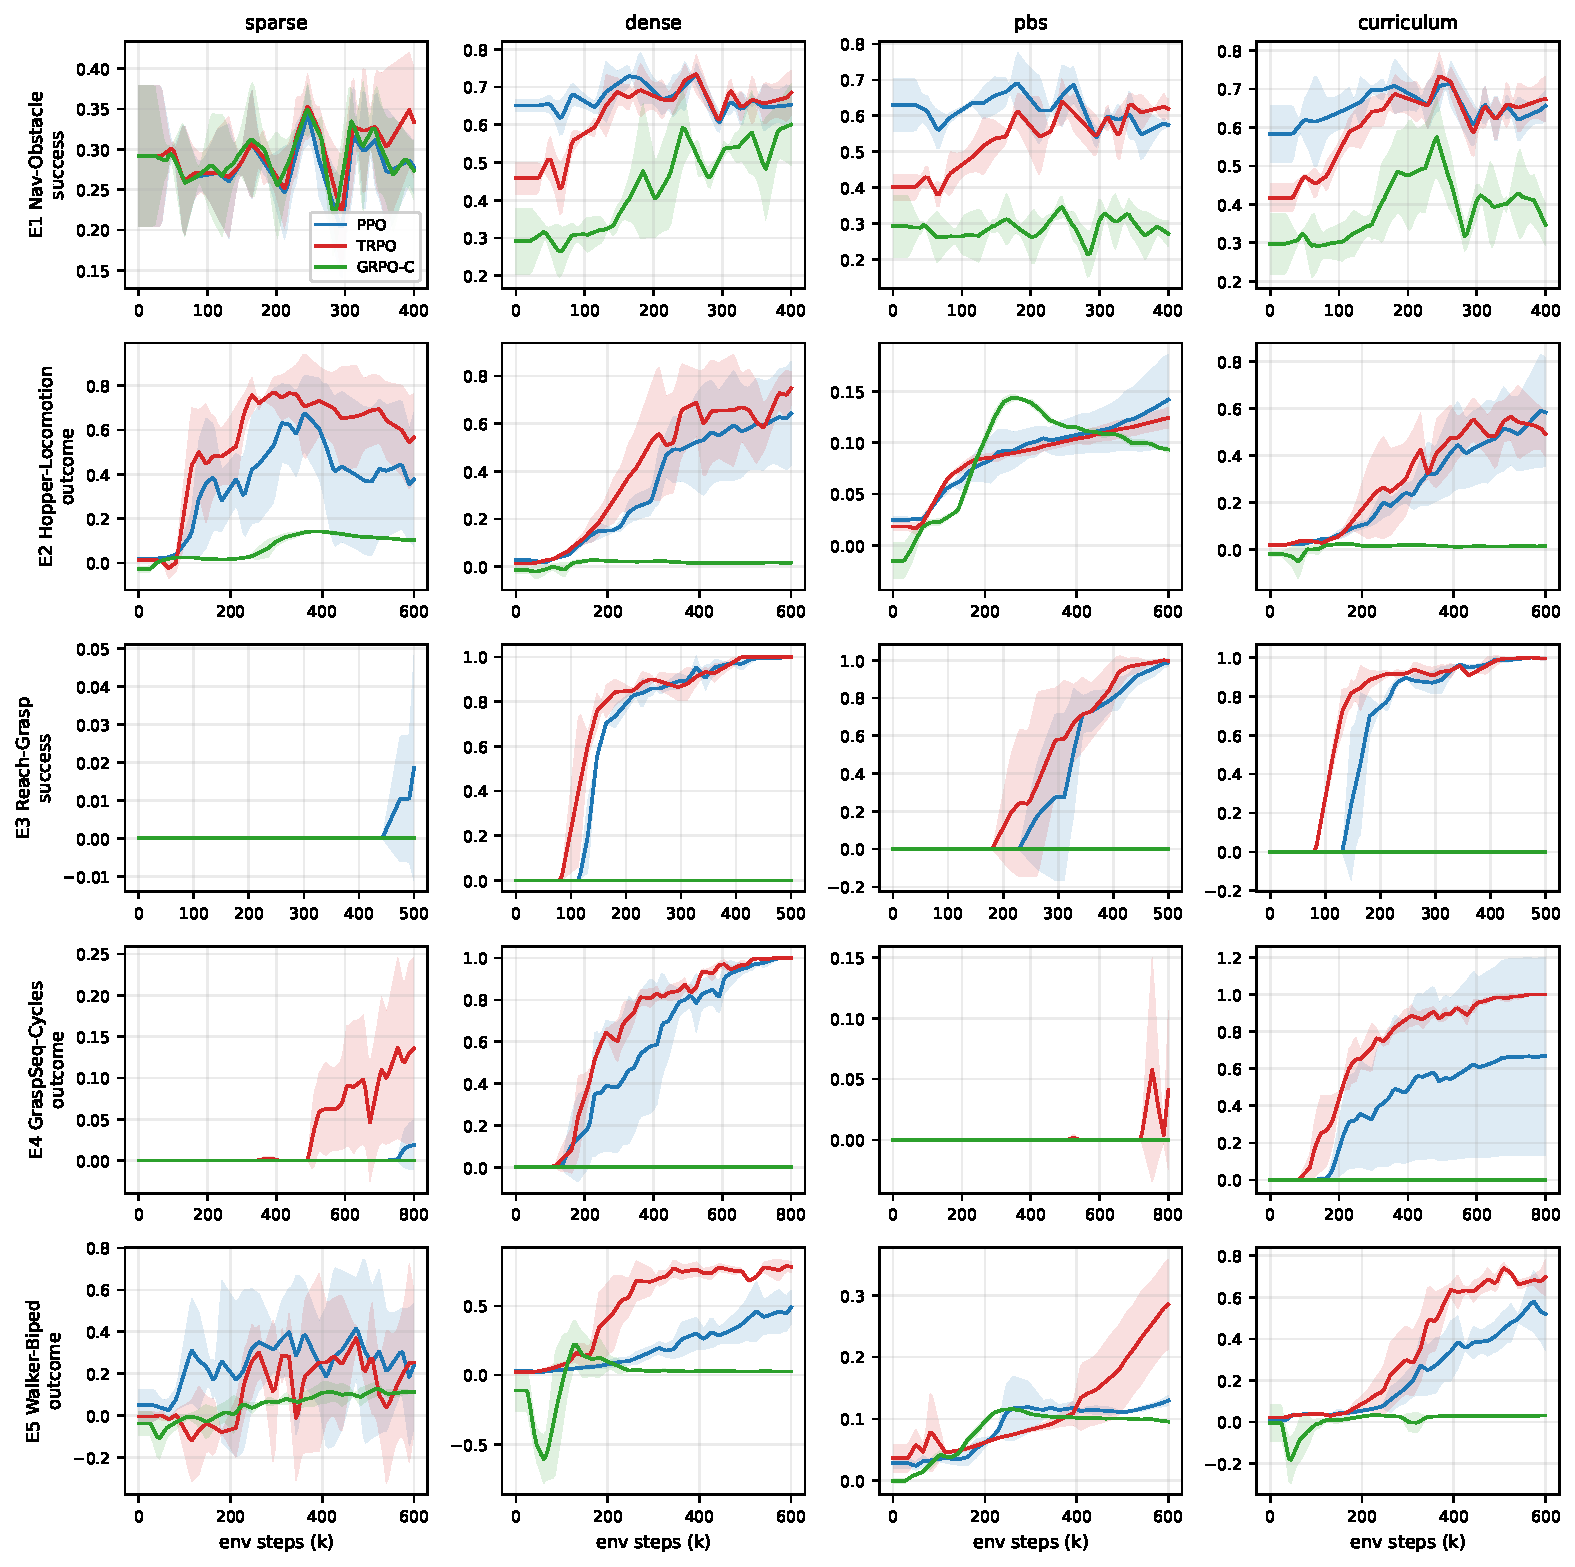
\includegraphics[width=\textwidth]{../../results/figs/reward_paradigm_grid.pdf}
\caption{Paradigm $\times$ task $\times$ algorithm learning curves
(\ppo{}-Clip, \trpo{}, \grpo{}; mean $\pm$95\% CI, 3 seeds).}
\label{fig:grid}
\end{figure*}

\subsection{Paradigm effects per task}
\textbf{E1 navigation} (final success, 3 seeds): dense and curriculum are
interchangeable for critic methods (\ppo{} 0.65/0.64, \trpo{} 0.67/0.66);
PBS costs 6--9 points (0.58/0.60); sparse collapses all of them to
0.29--0.32. Navigation rewards are naturally ``distance-shaped,'' so a
hand-designed potential adds little beyond dense progress terms, while
losing the event bonuses.
\textbf{E2 locomotion}: dense leads (\ppo{} 0.62, \trpo{} 0.68),
curriculum follows (0.55/0.53), \emph{sparse is workable} (0.41/0.61---%
\trpo{} under sparse reaching 0.61 is the paradigm study's surprise:
terminal displacement credit is clean credit), and \emph{PBS is
catastrophic} (0.13/0.12). The E2 potential $\phi=2v_x^{clip}
+0.5\,\mathrm{alive}+0.5y$ biases the discounted optimum toward
high-potential \emph{early} states under $\gamma=0.99$: the agent farms
the potential's alive/height terms rather than traveling---a live
demonstration that the Ng et al.\ invariance guarantee degenerates when
$\phi$ is not value-aligned and $\gamma<1$.
\textbf{E3 grasping}: dense $\approx$ curriculum $\approx$ PBS
(0.94--1.00 for all three critic methods) $\gg$ sparse (0.00--0.01).
Here the potential $\phi=-4d_{eo}+2\,\mathbb 1[\mathrm{grasp}]\min(h,0.18)$
encodes the task's own subgoal structure, so PBS behaves like the dense
terms it summarizes; only the fully sparse outcome starves credit
assignment across the reach--close--lift chain.

\subsection{Algorithm dependence}
The paradigm ranking depends on the optimizer's credit grain:
\grpo{} (episode-outcome baseline) is paradigm-insensitive on E3---all
paradigms end at 0.00---and on E1 it inverts the critic methods' sparse
pessimism only partially (sparse 0.29 $\approx$ dense 0.56$\to$curriculum
0.40). On E2, \grpo{} with sparse (0.11) beats \grpo{} with dense
(0.02): dense multi-term returns add \emph{within-group variance from
irrelevant terms} (effort, time), polluting the group baseline, while the
sparse outcome stream keeps groups comparable. Group baselines prefer
clean, low-dimensional outcome signals---the opposite of critic methods,
which thrive on dense per-step structure.

\subsection{Term audits}
Per-term telemetry (mean magnitudes over training) separates the three
dense designs: E1's return is dominated by the progress term (healthy);
E2's by the speed term with early fall penalties (healthy); E3's audit
exposed the flicker exploit of \S\ref{sec:hacking} (grasp-event term at
0.59/step $\approx$ 96\% of return magnitude before the fix, versus
$<$5\% after). We consider online term auditing a mandatory safety net
for engineered rewards.

\section{Case Study: Grasp-Flicker Reward Hacking}
\label{sec:hacking}
During library development the grasp dense paradigm originally paid a
per-step \emph{grasp-hold} bonus while the end-effector stayed near the
object. The resulting policy parked at the attach boundary and let
distance jitter flip the grasp state every step, farming the event stream
(term audit: grasp-event mean 0.59/step, dominating all task terms) while
never lifting. Two fixes restored task-aligned behaviour: (i) environment
hysteresis---attach below $0.04$\,m, hold until $0.06$\,m---removing the
flicker substrate; (ii) paying the grasp event once per episode. After the
fix the same algorithm reaches 95\%+ lift success. The general lesson:
\emph{event-type rewards must be rate-limited by design, and their audit
signature (sustained per-step frequency) monitored online}.

\section{Design Guidelines}
\label{sec:guidelines}
The theory (\S\ref{sec:theory}), the controlled study (\S\ref{sec:results})
and the case study (\S\ref{sec:hacking}) support the following guidelines.

\begin{enumerate}
\item \textbf{Start from the sparse task reward, then justify every added
term.} The sparse reward defines the task; every dense term is a hypothesis
about credit assignment that must pay for itself in sample efficiency or
final performance---and must be auditable. Our per-term telemetry makes
this a measurement, not a belief.
\item \textbf{Rate-limit every event-type bonus.} One-shot events
(grasp, milestone, stage clears) should fire at most once per episode or
carry an explicit refractory period; per-step event streams are farmable
(\S\ref{sec:hacking}).
\item \textbf{Prefer PBS when the potential is informative.} Potential-based
shaping is the only paradigm with a policy-invariance guarantee; it
converts a sparse task into a dense gradient without changing the apparent
task. Its limits: with $\gamma<1$ a hand-designed $\phi$ biases the
discounted optimum toward states of high $\phi$ early, and a $\phi$ no more
informative than the task signal adds nothing.
\item \textbf{Dense engineering must escape plateaus, not just descend
gradients.} A pure $\Delta(\text{goal quantity})$ term gives zero gradient
once partial progress stalls; milestone bonuses (or curriculum staging)
re-seed exploration. On E3 the plateau between grasp and lift stalled all
three algorithms until milestones were added.
\item \textbf{Match the paradigm to the optimizer's credit assignment
grain.} Critic-based methods (PPO/TRPO/SAC) exploit per-step dense signals;
group-outcome methods (GRPO/DAPO) only observe the episode return sum, so
(a) dense terms help them less per unit of design effort, and (b) they are
unexpectedly strong under pure sparse outcomes, where the group baseline
removes exactly the outcome-level variance that defeats sparse-reward
critic training.
\item \textbf{Curriculum is a task-difficulty instrument, not only a reward
instrument.} Scheduling obstacle counts, target speeds or spawn corridors
changes what the policy experiences; reward annealing changes only what it
is paid. The two interact: annealing reward to sparse while the task is
still at low difficulty produces a long degenerate phase.
\item \textbf{Audit online.} Log per-term means at training time. Signatures
of trouble: one term $>$80\% of total return magnitude sustained; event
terms firing at per-step frequency; success rate flat while return climbs
(the smoking gun of \S\ref{sec:hacking}).
\end{enumerate}

\section{Conclusion}
We formalized four reward paradigms, instantiated and audited twelve reward
functions across three robot tasks, and measured their interaction with
three optimizer families under a controlled protocol. The envelope is now
concrete: dense and curriculum dominate when credit structure matters;
PBS is a high-beta instrument---excellent when the potential mirrors
subgoal structure (grasping), destructive when it decorates a
velocity-style task under discounting (locomotion); sparse rewards are
viable for critic methods only with terminal credit as clean as
displacement; and group-outcome optimizers want sparse, low-dimensional
outcome streams, the opposite diet of critic methods. Each paradigm's
failure mode was caught not by final scores but by per-term audits---%
including a documented flicker-farming exploit---arguing for audits as
standard practice. The library, audits, and run logs are released
to make reward design a measured engineering discipline rather than
folklore.

\bibliographystyle{IEEEtran}
\begin{thebibliography}{12}
\bibitem{ng1999policy} A. Ng, D. Harada, S. Russell, ``Policy invariance
under reward transformations: Theory and application to reward shaping,''
in \emph{ICML}, 1999.
\bibitem{bengio2009curriculum} Y. Bengio et al., ``Curriculum learning,''
in \emph{ICML}, 2009.
\bibitem{shao2024grpo} Z. Shao et al., ``DeepSeekMath,''
\emph{arXiv:2402.03300}, 2024.
\bibitem{yu2025dapo} Q. Yu et al., ``DAPO,''
\emph{arXiv:2503.14476}, 2025.
\bibitem{schulman2017ppo} J. Schulman et al., ``Proximal policy
optimization algorithms,'' \emph{arXiv:1707.06347}, 2017.
\bibitem{schulman2015trpo} J. Schulman et al., ``Trust region policy
optimization,'' in \emph{ICML}, 2015.
\bibitem{wiewiora2003principled} E. Wiewiora, ``Potential-based shaping
and Q-value initialization are equivalent,'' \emph{JAIR}, 2003.
\bibitem{amodei2016concrete} D. Amodei et al., ``Concrete problems in AI
safety: Reward specification,'' \emph{arXiv:1606.06565}, 2016.
\bibitem{randlov1998bicycle} J. Randlov, P. Alstrom, ``Learning to drive a
bicycle using reinforcement learning and shaping,'' in \emph{ICML}, 1998.
\bibitem{eureka2023} Y. Ma et al., ``Eureka: Human-level reward design via
coding large language models,'' \emph{arXiv:2310.12931}, 2023.
\end{thebibliography}

\end{document}
